\section{Resultados}\label{sec:resultados}

\subsection{\label{sub:data}Datos}\label{subsec:label{sub:data}datos}

En esta secci�n, se incluyen los datos experimentales tomados en el laboratorio y sus errores asociados.

Las tablas~\ref{tab:1-t1-20},~\ref{tab:1-t1-45},~\ref{tab:2-t1-20} y~\ref{tab:2-t1-45} muestran
las mediciones del tiempo para las longitudes, �ngulos y masas especificadas.

\begin{table}[h!]
    \caption{Masa 1 - $20 \text{\textdegree}$ - Tiempo.}
    \label{tab:1-t1-20}
    \begin{centering}
        \begin{tabular}{|P{27px}|P{26px}P{26px}P{26px}|P{26px}P{26px}|}
            \hline
            $l$\,(mm)  & $t_1$\,(s) & $t_2$\,(s) & $t_3$\,(s) & $\langle t \rangle$\,(s) & $D_m$\,(s)                             \\
            \hline
            \csvreader[late after line= \\, /csv/separator=semicolon ]{./files/data/1-t-20_es.csv}{}% use head of csv as column names
            {\csvcolii & \csvcoliii & \csvcoliv  & \csvcolv   & \csvcolvi                & \csvcolvii}% specify your columns here
            \hline
        \end{tabular}
    \end{centering}
\end{table}

\begin{table}[h!]
    \caption{Masa 1 - $45 \text{\textdegree}$ - Tiempo.}
    \label{tab:1-t1-45}
    \begin{centering}
        \begin{tabular}{|P{27px}|P{26px}P{26px}P{26px}|P{26px}P{26px}|}
            \hline
            $l$\,(mm)  & $t_1$\,(s) & $t_2$\,(s) & $t_3$\,(s) & $\langle t \rangle$\,(s) & $D_m$\,(s)                             \\
            \hline
            \csvreader[late after line= \\, /csv/separator=semicolon ]{./files/data/1-t-45_es.csv}{}% use head of csv as column names
            {\csvcolii & \csvcoliii & \csvcoliv  & \csvcolv   & \csvcolvi                & \csvcolvii}% specify your columns here
            \hline
        \end{tabular}
    \end{centering}
\end{table}


Se contaron 20 oscilaciones para la masa 1 y 10 oscilaciones para la masa 2.

En cada tabla, se muestra la media de los 3 valores, o valor esperado de $t$, $\langle t \rangle$.
Tambi�n la dispersi�n de los datos  $D_m$, calculada como:
\begin{equation}
    D_m = \frac{x_{\text{m�x}} - x_{\text{m�n}}}{2}
\end{equation}




\begin{table}[h!]
    \caption{Masa 2 - $20 \text{\textdegree}$ - Tiempo.}
    \label{tab:2-t1-20}
    \begin{centering}
        \begin{tabular}{|P{27px}|P{26px}P{26px}P{26px}|P{26px}P{26px}|}
            \hline
            $l$\,(mm)  & $t_1$\,(s) & $t_2$\,(s) & $t_3$\,(s) & $\langle t \rangle$\,(s) & $D_m$\,(s)                             \\
            \hline
            \csvreader[late after line= \\, /csv/separator=semicolon ]{./files/data/2-t-20_es.csv}{}% use head of csv as column names
            {\csvcolii & \csvcoliii & \csvcoliv  & \csvcolv   & \csvcolvi                & \csvcolvii}% specify your columns here
            \hline
        \end{tabular}
    \end{centering}
\end{table}

\begin{table}[h!]
    \caption{Masa 2 - $45 \text{\textdegree}$ - Tiempo.}
    \label{tab:2-t1-45}
    \begin{centering}
        \begin{tabular}{|P{27px}|P{26px}P{26px}P{26px}|P{26px}P{26px}|}
            \hline
            $l$\,(mm)  & $t_1$\,(s) & $t_2$\,(s) & $t_3$\,(s) & $\langle t \rangle$\,(s) & $D_m$\,(s)                             \\
            \hline
            \csvreader[late after line= \\, /csv/separator=semicolon ]{./files/data/2-t-45_es.csv}{}% use head of csv as column names
            {\csvcolii & \csvcoliii & \csvcoliv  & \csvcolv   & \csvcolvi                & \csvcolvii}% specify your columns here
            \hline
        \end{tabular}
    \end{centering}
\end{table}

\FloatBarrier

\subsection{\label{sub:results}An�lisis}\label{subsec:label{sub:results}analisis}

\subsubsection{C�lculo de $T$}

Fij�ndonos en los valores obtenidos de la dispersi�n $D_m$, un valor razonable del error absoluto en la medici�n de los tiempos es $\pm 0.2\,s$.

Las tablas~\ref{tab:1-t3-20},~\ref{tab:1-t3-45},~\ref{tab:2-t3-20} y~\ref{tab:2-t3-45} muestran el periodo calculado a partir de los datos anteriores.

\begin{table}[h!]
    \caption{Masa 1 - 20\textdegree\;- Periodo.}
    \label{tab:1-t3-20}
    \begin{centering}
        \begin{tabular}{|P{56px}|P{67px}|P{67px}|}
            \hline
            $l$\,(mm)  & $t$\,(s)  & $T = t / n$\,(s)                       \\
            \hline
            \csvreader[late after line= \\, /csv/separator=semicolon ]{./files/data/1-t-20_es.csv}{}% use head of csv as column names
            {\csvcolii & \csvcolxi & \csvcolxii}% specify your columns here
            \hline
        \end{tabular}
    \end{centering}
\end{table}

\begin{table}[h!]
    \caption{Masa 1 - 45\textdegree\;- Periodo.}
    \label{tab:1-t3-45}
    \begin{centering}
        \begin{tabular}{|P{56px}|P{67px}|P{67px}|}
            \hline
            $l$\,(mm)  & $t$\,(s)  & $T = t / n$\,(s)                       \\
            \hline
            \csvreader[late after line= \\, /csv/separator=semicolon ]{./files/data/1-t-45_es.csv}{}% use head of csv as column names
            {\csvcolii & \csvcolxi & \csvcolxii}% specify your columns here
            \hline
        \end{tabular}
    \end{centering}
\end{table}

\begin{table}[h!]
    \caption{Masa 2 - 20\textdegree\;- Periodo.}
    \label{tab:2-t3-20}
    \begin{centering}
        \begin{tabular}{|P{56px}|P{67px}|P{67px}|}
            \hline
            $l$\,(mm)  & $t$\,(s)  & $T = t / n$\,(s)                       \\
            \hline
            \csvreader[late after line= \\, /csv/separator=semicolon ]{./files/data/2-t-20_es.csv}{}% use head of csv as column names
            {\csvcolii & \csvcolxi & \csvcolxii}% specify your columns here
            \hline
        \end{tabular}
    \end{centering}
\end{table}

\begin{table}[h!]
    \caption{Masa 2 - 45\textdegree\;- Periodo.}
    \label{tab:2-t3-45}
    \begin{centering}
        \begin{tabular}{|P{56px}|P{67px}|P{67px}|}
            \hline
            $l$\,(mm)  & $t$\,(s)  & $T = t / n$\,(s)                       \\
            \hline
            \csvreader[late after line= \\, /csv/separator=semicolon ]{./files/data/2-t-45_es.csv}{}% use head of csv as column names
            {\csvcolii & \csvcolxi & \csvcolxii}% specify your columns here
            \hline
        \end{tabular}
    \end{centering}
\end{table}

\FloatBarrier


Observamos que el periodo $T$ es ligeramente mayor para el �ngulo de 45\textdegree\;que para el de 20\textdegree.

Observamos tambi�n que el periodo $T$ es el mismo para ambas masas. $T$ es independiente de $m$ porque en un campo gravitatorio
todos los cuerpos adquieren la misma aceleraci�n.

\subsubsection{$T$ frente a $\sqrt{l}$}

Las figuras~\ref{fig:1-20-1},~\ref{fig:1-45-1},~\ref{fig:2-20-1} y~\ref{fig:2-45-1} muestran las gr�ficas del periodo $T$
frente a la ra�z cuadrada de la longitud $\sqrt{l}$.
\footnote{En las figuras se emplea la notaci�n anglosajona, donde se utiliza el punto como separador de decimales.
}.

\begin{figure}[h!]
    \begin{center}
        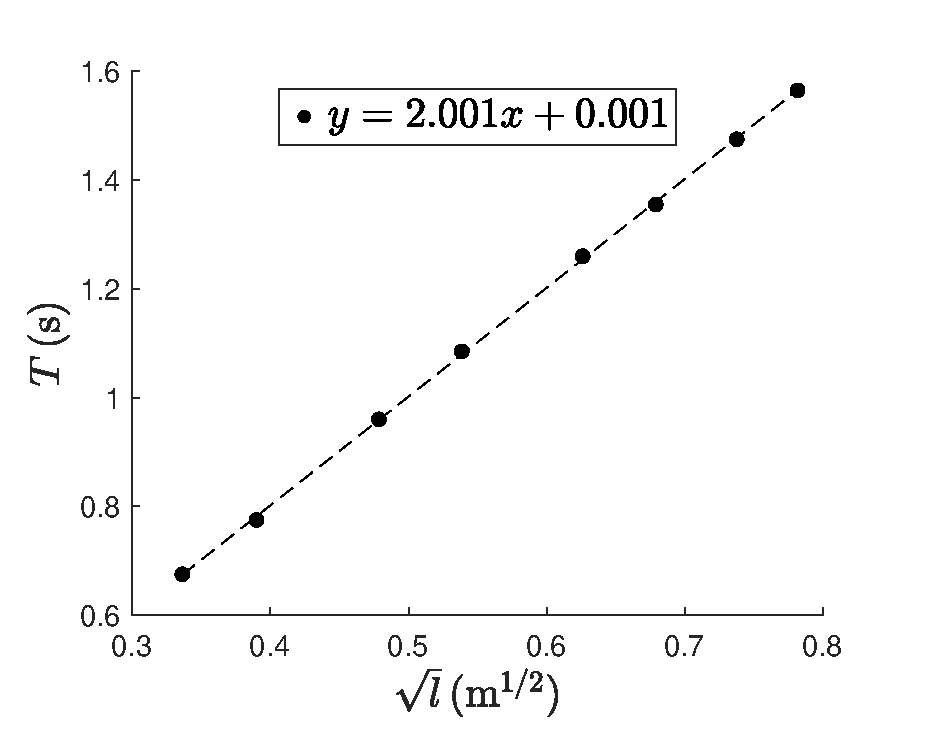
\includegraphics[width=0.8\columnwidth]{files/images/1-20-1}
    \end{center}
    \caption{Masa 1 - 20\textdegree\;- $T$ frente a $\sqrt {l}$.}
    \label{fig:1-20-1}
\end{figure}

\begin{figure}[h!]
    \begin{center}
        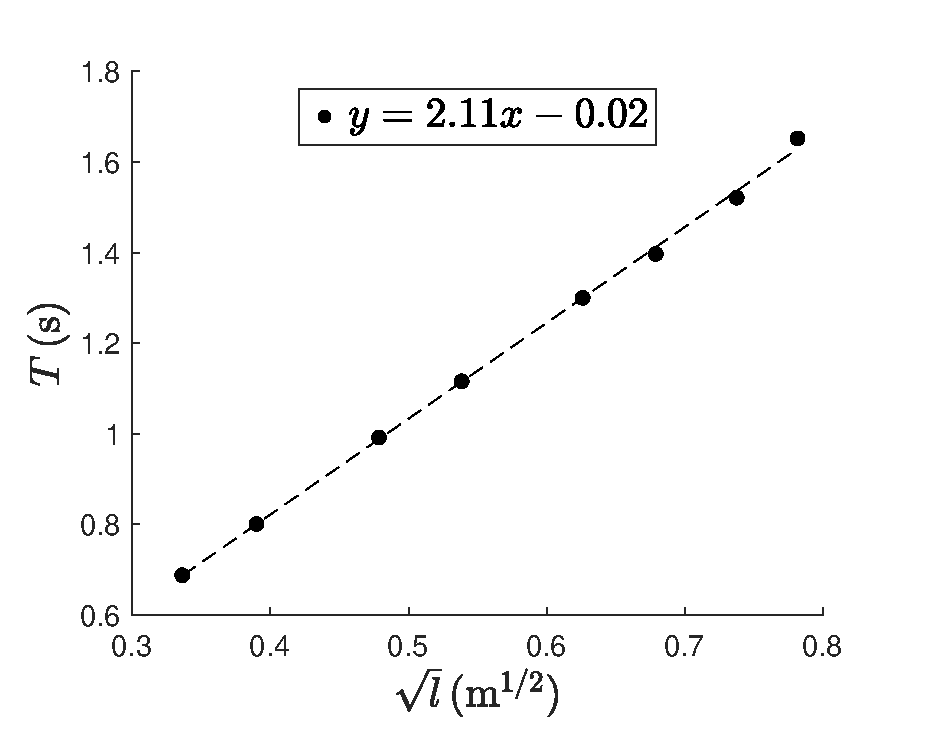
\includegraphics[width=0.8\columnwidth]{files/images/1-45-1}
    \end{center}
    \caption{Masa 1 - 45\textdegree\;- $T$ frente a $\sqrt {l}$.}
    \label{fig:1-45-1}
\end{figure}

\begin{figure}[h!]
    \begin{center}
        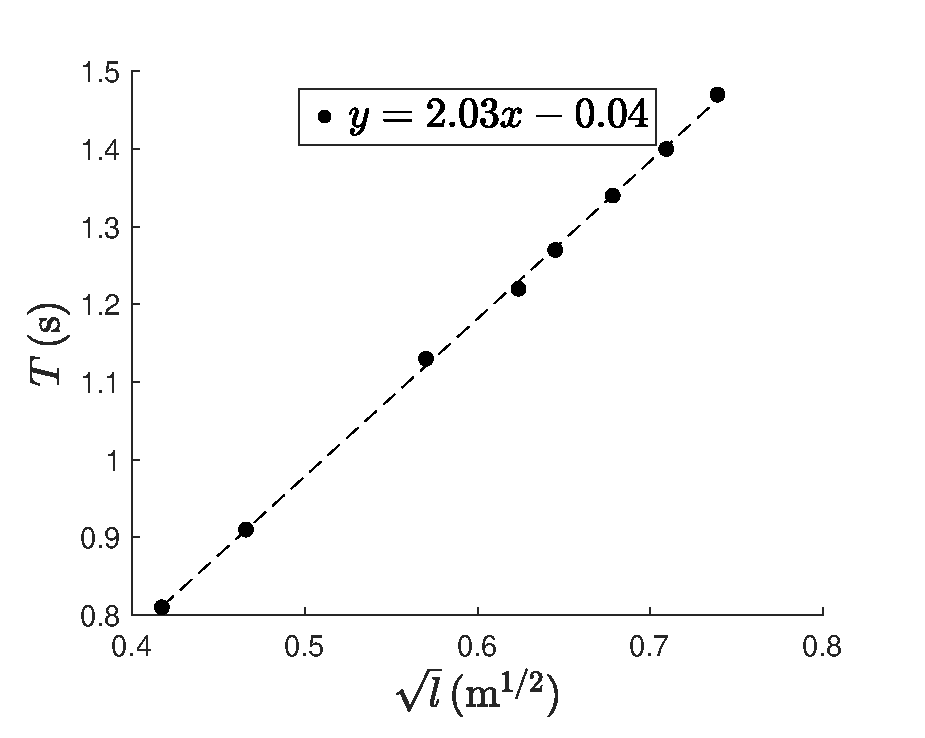
\includegraphics[width=0.8\columnwidth]{files/images/2-20-1}
    \end{center}
    \caption{Masa 2 - 20\textdegree\;- $T$ frente a $\sqrt {l}$.}
    \label{fig:2-20-1}
\end{figure}

\begin{figure}[h!]
    \begin{center}
        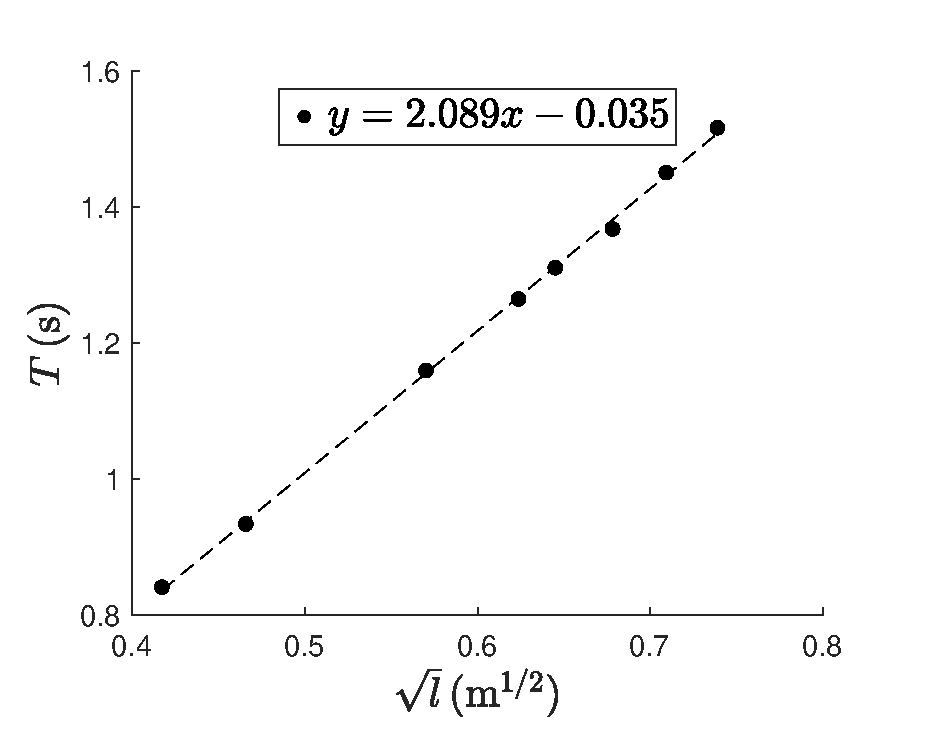
\includegraphics[width=0.8\columnwidth]{files/images/2-45-1}
    \end{center}
    \caption{Masa 2 - 45\textdegree\;- $T$ frente a $\sqrt {l}$.}
    \label{fig:2-45-1}
\end{figure}

\FloatBarrier

A partir de la pendiente de las gr�ficas~\ref{fig:1-20-1},~\ref{fig:1-45-1},~\ref{fig:2-20-1} y~\ref{fig:2-45-1}, podemos
calcular el valor de la aceleraci�n de la gravedad $g$.
El error que aparece en el valor de la pendiente $a$ es la desviaci�n est�ndar del ajuste de m�nimos cuadrados.

La tabla~\ref{tab:g} muestra los valores calculados de $g$.

\begin{table}[h!]
    \caption{$g$ calculada a partir de la recta $T$ frente a $\sqrt {l}$.}
    \label{tab:g}
    \begin{centering}
        \begin{tabular}{|P{56px}|P{67px}|P{67px}|}
            \hline
            & $a\;\text{(s/m$^{1/2}$)}$ & $g\;\text{(m/s$^2$)}$ \\
            \hline
            Masa 1, 20\textdegree & 2,001 \pm\; 0,011         & 9,86 \pm\; 0,11       \\
            Masa 1, 45\textdegree & 2,11 \pm\; 0,03           & 8,9 \pm\; 0,3         \\
            Masa 2, 20\textdegree & 2,03 \pm\; 0,02           & 9,58 \pm\; 0,19       \\
            Masa 2, 45\textdegree & 2,10 \pm\; 0,03           & 9,0 \pm\; 0,3         \\
            \hline
        \end{tabular}
    \end{centering}
\end{table}

Observamos que la pendiente de la recta $T$ frente a $\sqrt {l}$ es mayor para �ngulos grandes, y esto a su vez resulta en un valor de
$g$ m�s peque�o.

\FloatBarrier

\subsubsection{$l$ frente a $T^2$}

De modo similar, las figuras~\ref{fig:1-20-2},~\ref{fig:1-45-2},~\ref{fig:2-20-2} y~\ref{fig:2-45-2} muestran la representaci�n
de la longitud $l$ frente al periodo al cuadrado $T^2$.

\begin{figure}[h!]
    \begin{center}
        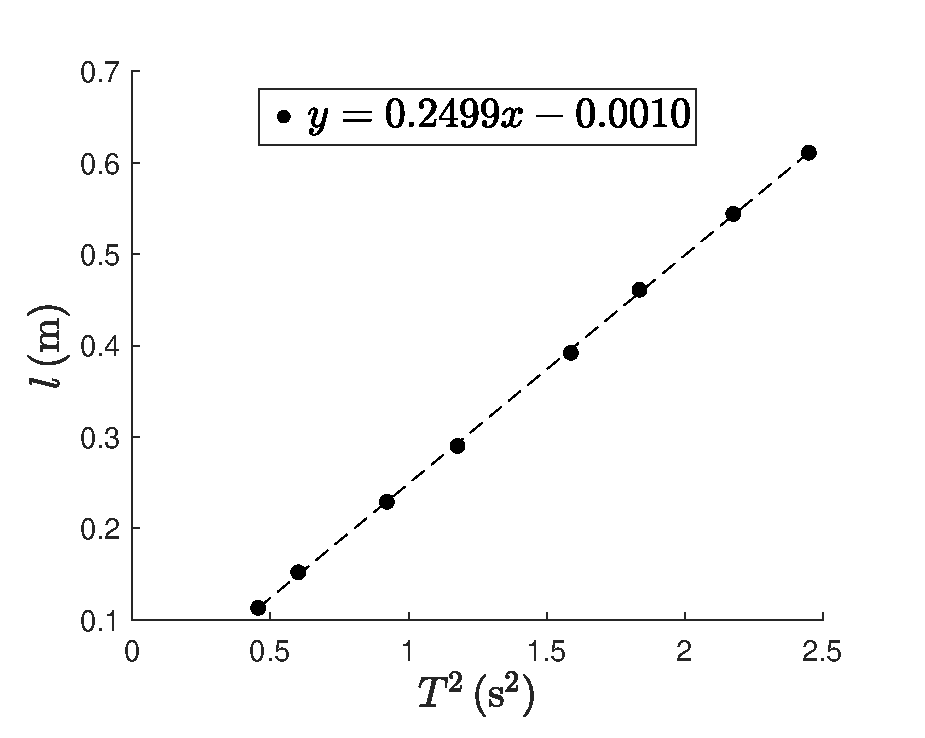
\includegraphics[width=0.8\columnwidth]{files/images/1-20-2}
    \end{center}
    \caption{Masa 1 - 20\textdegree\;- $l$ frente a $T^2$.}
    \label{fig:1-20-2}
\end{figure}

\begin{figure}[h!]
    \begin{center}
        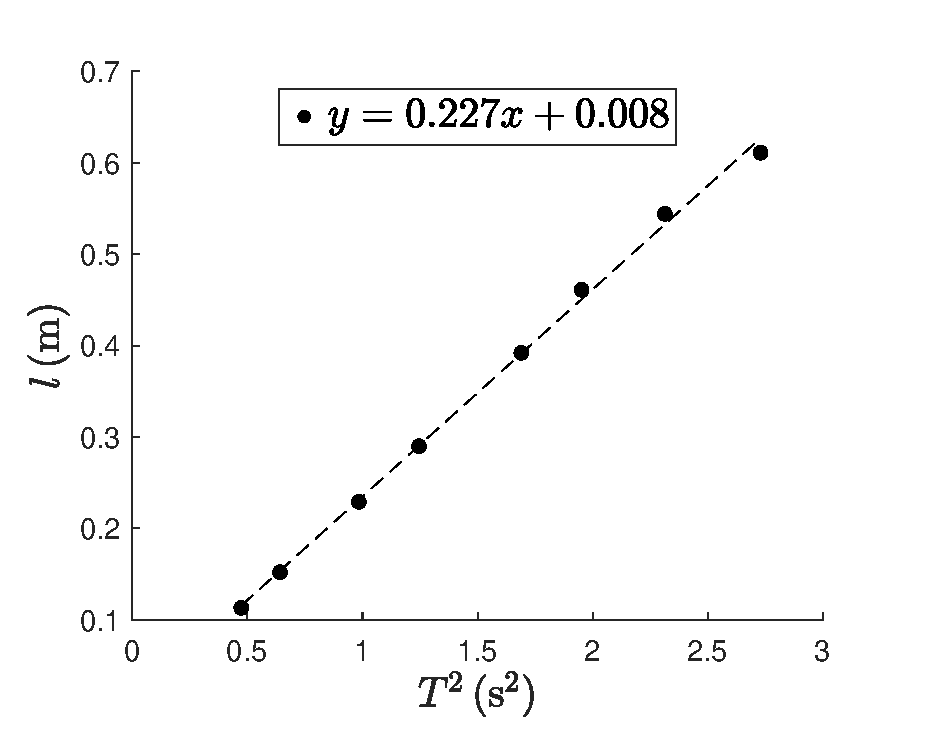
\includegraphics[width=0.8\columnwidth]{files/images/1-45-2}
    \end{center}
    \caption{Masa 1 - 45\textdegree\;- $l$ frente a $T^2$.}
    \label{fig:1-45-2}
\end{figure}

\begin{figure}[h!]
    \begin{center}
        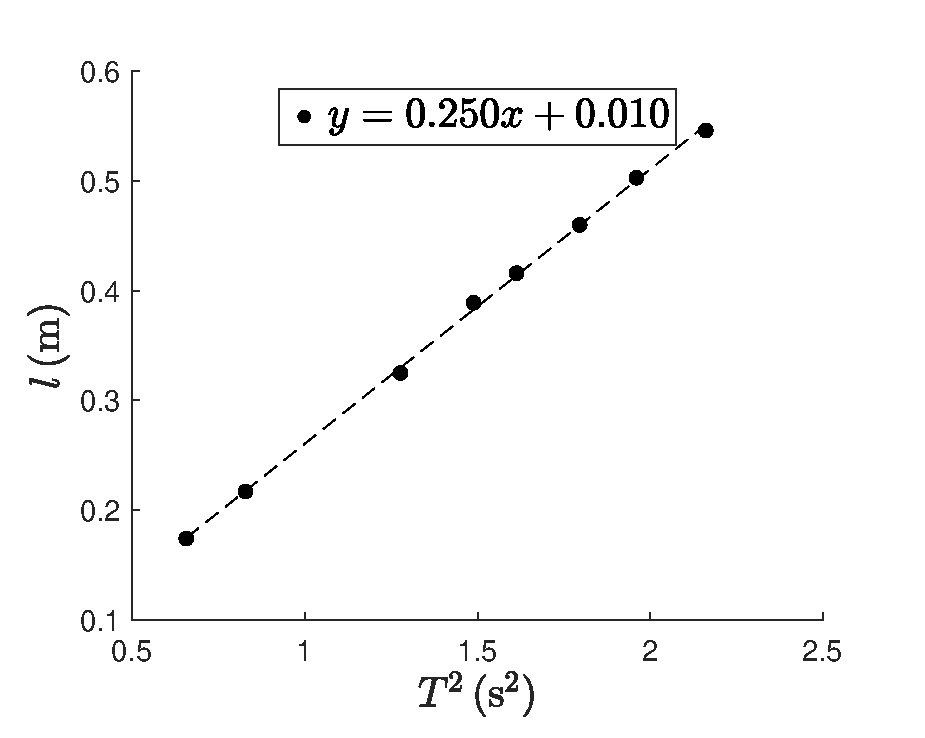
\includegraphics[width=0.8\columnwidth]{files/images/2-20-2}
    \end{center}
    \caption{Masa 2 - 20\textdegree\;- $l$ frente a $T^2$.}
    \label{fig:2-20-2}
\end{figure}

\begin{figure}[h!]
    \begin{center}
        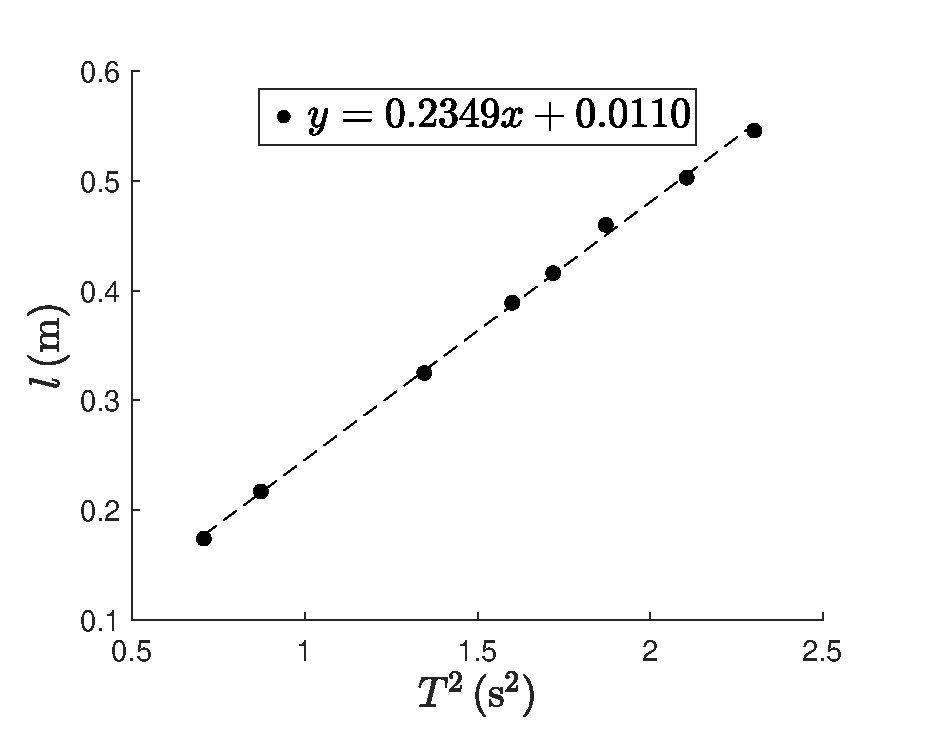
\includegraphics[width=0.8\columnwidth]{files/images/2-45-2}
    \end{center}
    \caption{Masa 2 - 45\textdegree\;- $l$ frente a $T^2$.}
    \label{fig:2-45-2}
\end{figure}

\FloatBarrier

A partir de la pendiente $a$ de las gr�ficas~\ref{fig:1-20-2},~\ref{fig:1-45-2},~\ref{fig:2-20-2} y~\ref{fig:2-45-2},
calculamos de nuevo $g$.

\begin{table}[h!]
    \caption{$g$ calculada a partir de la recta $l$ frente a $T^2$.}
    \label{tab:g2}
    \begin{centering}
        \begin{tabular}{|P{50px}|P{71px}|P{69px}|}
            \hline
            & $a\;\text{(s/m$^{1/2}$)}$ & $g\;\text{(m/s$^2$)}$ \\
            \hline
            Masa 1, 20\textdegree & 0,2499 \pm\; 0,0014       & 9,87 \pm\; 0,06       \\
            Masa 1, 45\textdegree & 0,227 \pm\; 0,004         & 8,96 \pm\; 0,16       \\
            Masa 2, 20\textdegree & 0,250 \pm\; 0,003         & 9,87 \pm\; 0,12       \\
            Masa 2, 45\textdegree & 0,233 \pm\; 0,003         & 9,20 \pm\; 0,12       \\
            \hline
        \end{tabular}
    \end{centering}
\end{table}

\FloatBarrier

Tanto en esta secci�n como en la anterior, los resultados para ambas masas son similares, como era de esperar.

\subsubsection{$l$ frente a $T$}

Por �ltimo, representamos la longitud $l$ frente al periodo $T$ en escala log-log en las
gr�ficas~\ref{fig:1-20-3},~\ref{fig:1-45-3},~\ref{fig:2-20-3} y~\ref{fig:2-45-3}.

\begin{figure}[h!]
    \begin{center}
        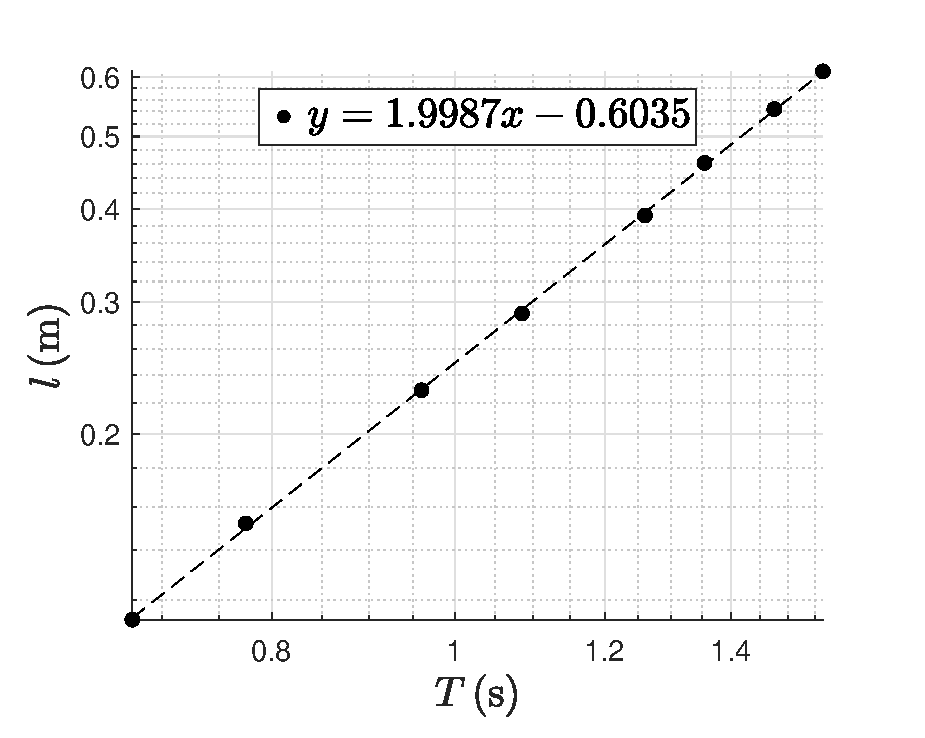
\includegraphics[width=0.8\columnwidth]{files/images/1-20-3}
    \end{center}
    \caption{Masa 1 - 20\textdegree\;- $l$ frente a $T$.}
    \label{fig:1-20-3}
\end{figure}

\begin{figure}[h!]
    \begin{center}
        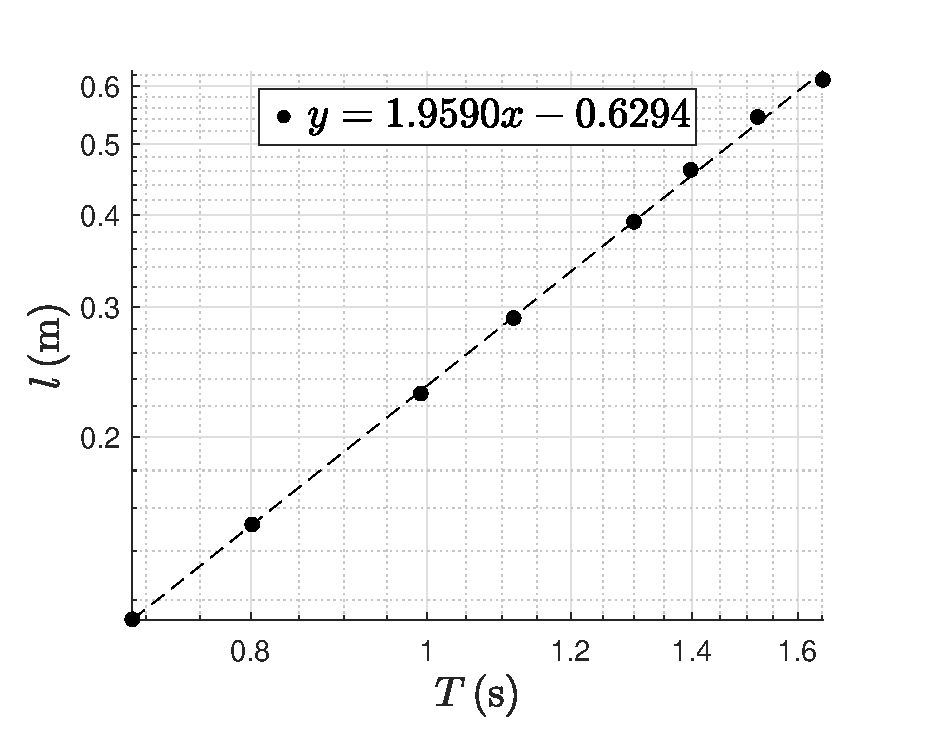
\includegraphics[width=0.8\columnwidth]{files/images/1-45-3}
    \end{center}
    \caption{Masa 1 - 45\textdegree\;- $l$ frente a $T$.}
    \label{fig:1-45-3}
\end{figure}

\begin{figure}[h!]
    \begin{center}
        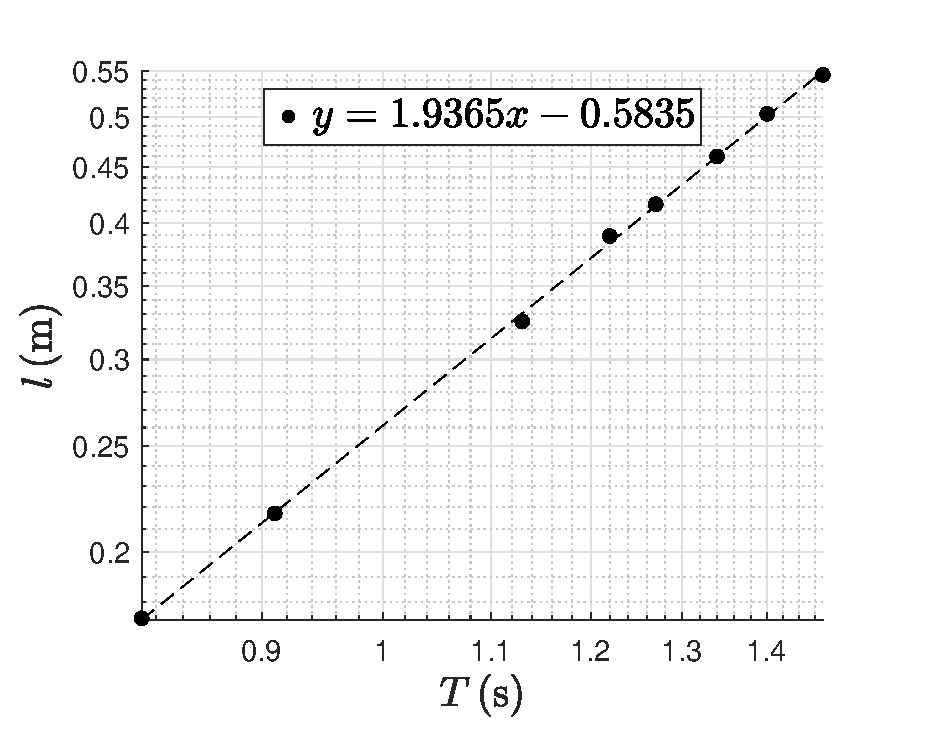
\includegraphics[width=0.8\columnwidth]{files/images/2-20-3}
    \end{center}
    \caption{Masa 2 - 20\textdegree\;- $l$ frente a $T$.}
    \label{fig:2-20-3}
\end{figure}

\begin{figure}[h!]
    \begin{center}
        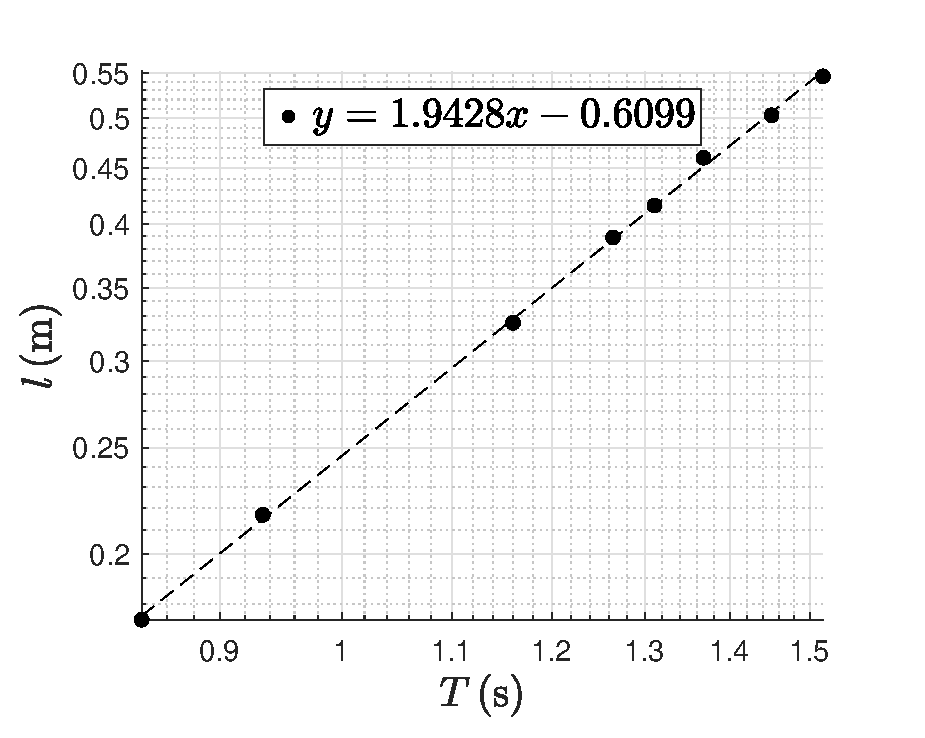
\includegraphics[width=0.8\columnwidth]{files/images/2-45-3}
    \end{center}
    \caption{Masa 2 - 45\textdegree\;- $l$ frente a $T$.}
    \label{fig:2-45-3}
\end{figure}

\FloatBarrier

Los puntos ($T_i$, $l_i$) en escala logar�tmica se distribuyen en una recta.

Una funci�n del tipo $Y = \alpha \, X^q$ en una representaci�n doblemente logar�tmica aparece
como una l�nea recta de pendiente igual a $q$, ya que tomando logaritmos:
\begin{equation*}
    \log_{10} Y = \log_{10} \alpha + q\,\log_{10} X
\end{equation*}

Por tanto, podemos deducir la ecuaci�n~\ref{eq:1} a partir de los valores de la pendiente y la intersecci�n
de las rectas en~\ref{fig:1-20-3},~\ref{fig:1-45-3},~\ref{fig:2-20-3} y~\ref{fig:2-45-3}.

Concretamente: $q = 2$ y $\alpha = g / 4\pi^2$.





